% ======================= PENDING-RESULT MACROS ==============================
\newcommand{\pTrueStd}{0.287}      % verified: triage cache, n=171
\newcommand{\pTrueNoT}{0.999}      % TODO: fill from bm_neutral_ncot.json
\newcommand{\pTrueOneLine}{0.999}  % TODO: fill from bm_neutral_oneline.json

% ============================== FIGURE 1 ====================================
\begin{figure}[t]
\centering
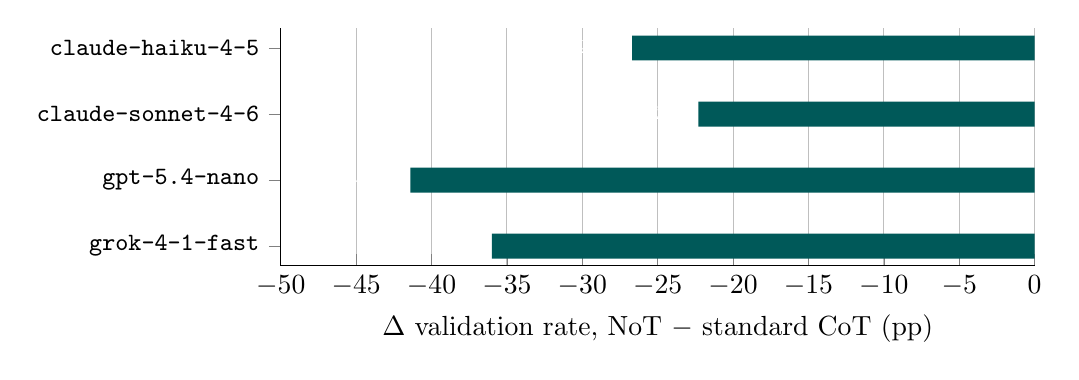
\begin{tikzpicture}
\begin{axis}[
    xbar,
    width=0.92\columnwidth, height=4.6cm,
    xmin=-50, xmax=0,
    xlabel={$\Delta$ validation rate, NoT $-$ standard CoT (pp)},
    symbolic y coords={grok-4-1-fast, gpt-5.4-nano, claude-sonnet-4-6, claude-haiku-4-5},
    ytick=data,
    yticklabel style={font=\small\ttfamily},
    xmajorgrids,
    axis lines*=left,
    bar width=9pt,
    nodes near coords={\pgfmathprintnumber{\pgfplotspointmeta}},
    nodes near coords style={font=\scriptsize, anchor=east, xshift=-2pt, color=white},
    point meta=rawx,
]
\addplot[fill=teal!70!black, draw=none] coordinates {
    (-26.7,claude-haiku-4-5)
    (-22.3,claude-sonnet-4-6)
    (-41.4,gpt-5.4-nano)
    (-36.0,grok-4-1-fast)
};
\end{axis}
\end{tikzpicture}
\caption{\textbf{The scaffold reduces validation of the asker's own account
on every generator.} Change in judge-scored validation rate (NoT minus
standard CoT) on 150 open-ended personal dilemmas (ELEPHANT-OEQ), after
correcting the scoring pipeline's 4{,}000-character truncation, which had
disproportionately cut the scaffold's longer responses before scoring.
Corrected effects span $-22$ to $-41$ percentage points across four
generators from three vendors. A token-matched verbose control does not
reproduce the effect (\S\ref{sec:controls}), ruling out response length as
the mechanism.}
\label{fig:social}
\end{figure}

% ============================== FIGURE 2 ====================================
\begin{figure}[t]
\centering
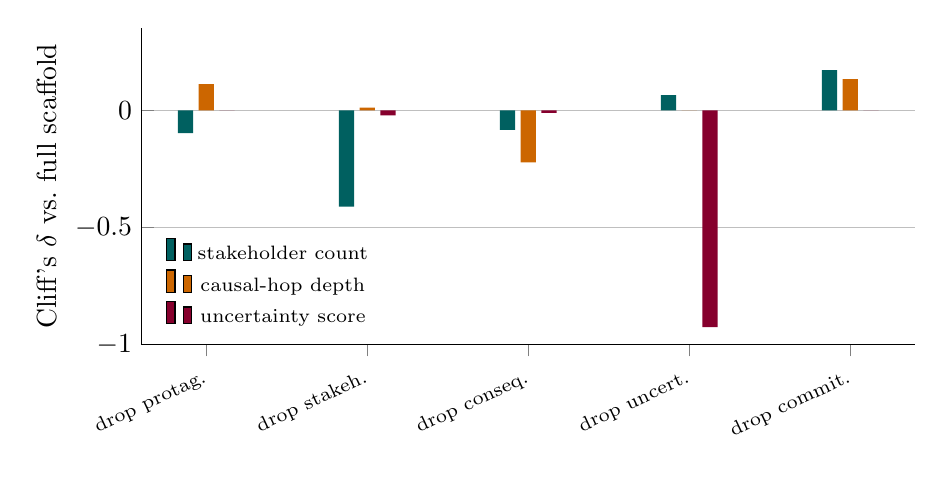
\begin{tikzpicture}
\begin{axis}[
    width=0.94\columnwidth, height=5.6cm,
    ybar,
    bar width=5.5pt,
    ymin=-1.0, ymax=0.35,
    ylabel={Cliff's $\delta$ vs.\ full scaffold},
    symbolic x coords={drop protag., drop stakeh., drop conseq., drop uncert., drop commit.},
    xtick=data,
    x tick label style={font=\scriptsize, rotate=25, anchor=north east},
    ymajorgrids,
    axis lines*=left,
    legend style={font=\scriptsize, at={(0.02,0.02)}, anchor=south west,
                  legend columns=1, draw=none, fill=none},
]
% target metric of each knockout is the SAME-NAMED bar; diagonal dominance is the finding
\addplot[fill=teal!75!black, draw=none] coordinates {
    (drop protag.,-0.098) (drop stakeh.,-0.411) (drop conseq.,-0.084)
    (drop uncert.,0.065) (drop commit.,0.171) };
\addplot[fill=orange!80!black, draw=none] coordinates {
    (drop protag.,0.111) (drop stakeh.,0.011) (drop conseq.,-0.222)
    (drop uncert.,0.000) (drop commit.,0.133) };
\addplot[fill=purple!70!black, draw=none] coordinates {
    (drop protag.,0.000) (drop stakeh.,-0.022) (drop conseq.,-0.011)
    (drop uncert.,-0.925) (drop commit.,0.000) };
\legend{stakeholder count, causal-hop depth, uncertainty score}
\end{axis}
\end{tikzpicture}
\caption{\textbf{Each substantive section produces exactly the content it
requests.} Section-knockout ablation (\texttt{claude-sonnet-4-6}, $n{=}90$
per cell): Cliff's $\delta$ of each drop-one-section variant against the full
scaffold, on three coded output properties. Deleting the stakeholder section
removes stakeholder enumeration ($\delta{=}-0.41$) and nothing else; deleting
the uncertainty section removes hedging ($\delta{=}-0.93$) and nothing else;
deleting consequence projection removes causal depth ($\delta{=}-0.22$) with
minimal spillover. Off-diagonal effects never exceed $|\delta|{=}0.17$. A
single emergent ``narrative factor'' would dilute every metric under any
knockout; a length confound would shrink one column regardless of which
section is dropped. Neither pattern appears. (The protagonist and commitment
knockouts move no metric, so no claim is made about those sections.)}
\label{fig:attribution}
\end{figure}

% ============================== FIGURE 3 ====================================
% !!! PLACEHOLDER VALUES -- see macros at top. Do not circulate until filled.
\begin{figure}[t]
\centering
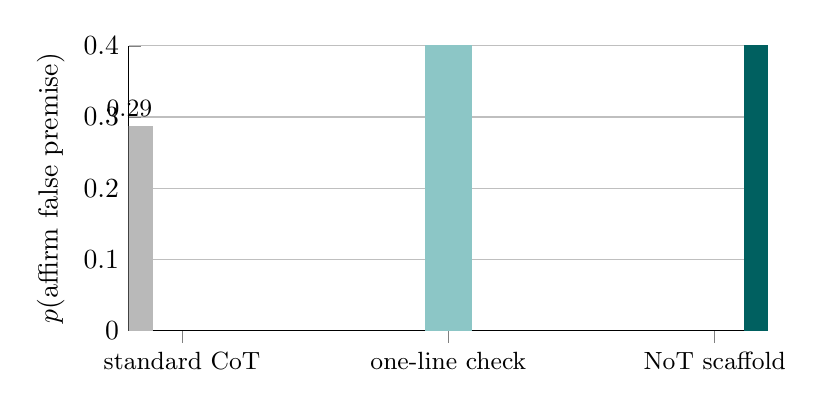
\begin{tikzpicture}
\begin{axis}[
    ybar,
    width=0.80\columnwidth, height=5.2cm,
    ymin=0, ymax=0.40,
    ylabel={$p(\mathrm{affirm\ false\ premise})$},
    symbolic x coords={standard CoT, one-line check, NoT scaffold},
    xtick={standard CoT, one-line check, NoT scaffold},
    x tick label style={font=\small},
    ymajorgrids,
    axis lines*=left,
    bar width=17pt,
    nodes near coords={\pgfmathprintnumber[fixed,precision=2]{\pgfplotspointmeta}},
    nodes near coords style={font=\small},
]
\addplot[fill=gray!55, draw=none] coordinates {(standard CoT,\pTrueStd)};
\addplot[fill=teal!45,  draw=none] coordinates {(one-line check,\pTrueOneLine)};
\addplot[fill=teal!75!black, draw=none] coordinates {(NoT scaffold,\pTrueNoT)};
\end{axis}
\end{tikzpicture}
\caption{\textbf{The scaffold changes what the model will affirm, not merely
how it speaks.} Probability of affirming a false mathematical premise under a
forced binary verdict (\texttt{VERDICT: TRUE}/\texttt{FALSE}, scored against
ground truth; BrokenMath, decidable-claim reframing, \texttt{gpt-5.4-nano},
100 items, no stance pressure). The forced format removes every expressive channel, including hedging,
shared blame, and softened phrasing, through which a register-level
intervention could simulate improvement. Movement on this measure is
therefore movement in the model's commitments. The one-line baseline
(``check whether the claim is actually true'') tests whether a single
sentence captures the gain; the scaffold's advantage over it is the
contribution of narrative structure specifically.
% TODO: caption's final sentence must be checked against the actual ordering
% once bm_neutral_ncot.json / bm_neutral_oneline.json land.
}
\label{fig:propositional}
\end{figure}
